\documentclass[journal, onecolumn]{IEEEtran}
\usepackage[english, spanish]{babel}
\usepackage[sorting=none]{biblatex}
\bibliography{ref.bib}
\usepackage{amsmath, amsfonts, amsthm}
\usepackage{hyperref, url}
\usepackage{graphicx}
\usepackage{fancyhdr, last page}
\usepackage{siunitx}
\usepackage{anyfontsize}
\usepackage{csquotes}
\usepackage{xcolor}
\usepackage[affil-sl]{authblk}
\usepackage[spanish]{cleveref}
\AtBeginDocument{\decimalpoint}
\usepackage{matlab}

\graphicspath{{./blocks_media/}}

\hypersetup{
    colorlinks=true,
    linkcolor=black,
    urlcolor=blue,
    pdftitle={Block Reduction - JL}
}
\urlstyle{same}
\sisetup{separate-uncertainty}

\begin{document}

\title{Función de Transferencia Figura 6 \\ Taller de Bloques con MATLAB}

\author[*]{Julian L. Avila
    \thanks{Julian Avila: 20212107030}}
\author[*]{Laura Y. Herrera
    \thanks{Laura Herrera: 20212107011}}

\affil[*]{Programa Académico de Física\\
    Universidad Distrital Francisco José de Caldas}

\markboth{}
{Shell \MakeLowercase{\textit{et al.}}: Bare Demo of IEEEtran.cls for IEEE Journals}

\maketitle
\section{Linea de Comandos}

\begin{matlabcode}
g1 = tf(1, [1 10]);
g2 = tf(1, [1 1]);
g3 = tf([1 0 1], [1 4 4]);
g4 = tf([1 1], [1 6]);
h1 = tf([1 1], [1 2]);
h2 = 2;
h3 = 1;

gf1 = feedback(series(g3, g4), h1);
gf2 = feedback(series(gf1, g2), h2 / g4);
t = feedback(series(gf2, g1), h3);

t = minreal(t);
zpk(t)
\end{matlabcode}
\begin{matlaboutput}
ans =

                        0.5 (s+2) (s+1) (s^2 + 1)
  -----------------------------------------------------------------------
  (s+9.914) (s+1.907) (s^2 + 1.224s + 1.053) (s^2 + 5.954s + 18.39)

Continuous-time zero/pole/gain model.
Model Properties
\end{matlaboutput}
\begin{matlabcode}

figure;
subplot(2, 2, 1); step(t); title('Step Response'); grid on;
subplot(2, 2, 2); impulse(t); title('Impulse Response'); grid on;
subplot(2, 2, 3); bode(t); title('Bode Plot'); grid on;
subplot(2, 2, 4); pzmap(t); title('Pole-Zero Map'); grid on;
\end{matlabcode}
\begin{center}
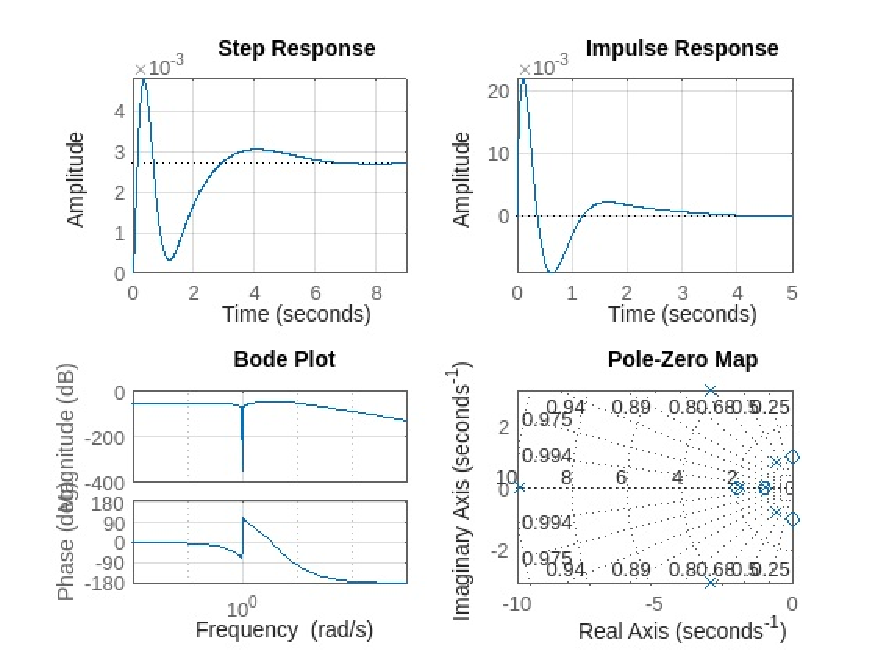
\includegraphics[width=\maxwidth{56.196688409433015em}]{figure_0.pdf}
\end{center}

\section{Simulink}
\begin{matlabcode}
[num, den] = linmod('Bloque_figura6')
\end{matlabcode}
\begin{matlaboutput}
num = 1x7
         0         0    0.5000    1.5000    1.5000    1.5000    1.0000

den = 1x7
    1.0000   19.0000  130.5000  480.5000  865.0000  773.0000  366.0000

\end{matlaboutput}
\begin{matlabcode}
GT=tf(num, den)
\end{matlabcode}
\begin{matlaboutput}
GT =

            0.5 s^4 + 1.5 s^3 + 1.5 s^2 + 1.5 s + 1
  ------------------------------------------------------------
  s^6 + 19 s^5 + 130.5 s^4 + 480.5 s^3 + 865 s^2 + 773 s + 366

Continuous-time transfer function.
Model Properties
\end{matlaboutput}
\begin{matlabcode}

GT = minreal(GT)
\end{matlabcode}
\begin{matlaboutput}
GT =

            0.5 s^4 + 1.5 s^3 + 1.5 s^2 + 1.5 s + 1
  ------------------------------------------------------------
  s^6 + 19 s^5 + 130.5 s^4 + 480.5 s^3 + 865 s^2 + 773 s + 366

Continuous-time transfer function.
Model Properties
\end{matlaboutput}
\begin{matlabcode}
zpk(GT)
\end{matlabcode}
\begin{matlaboutput}
ans =

                      0.5 (s+2) (s+1) (s^2 + 1)
  -----------------------------------------------------------------
  (s+9.914) (s+1.907) (s^2 + 1.224s + 1.053) (s^2 + 5.954s + 18.39)

Continuous-time zero/pole/gain model.
Model Properties
\end{matlaboutput}

\begin{figure}[htbp!]
\begin{center}
    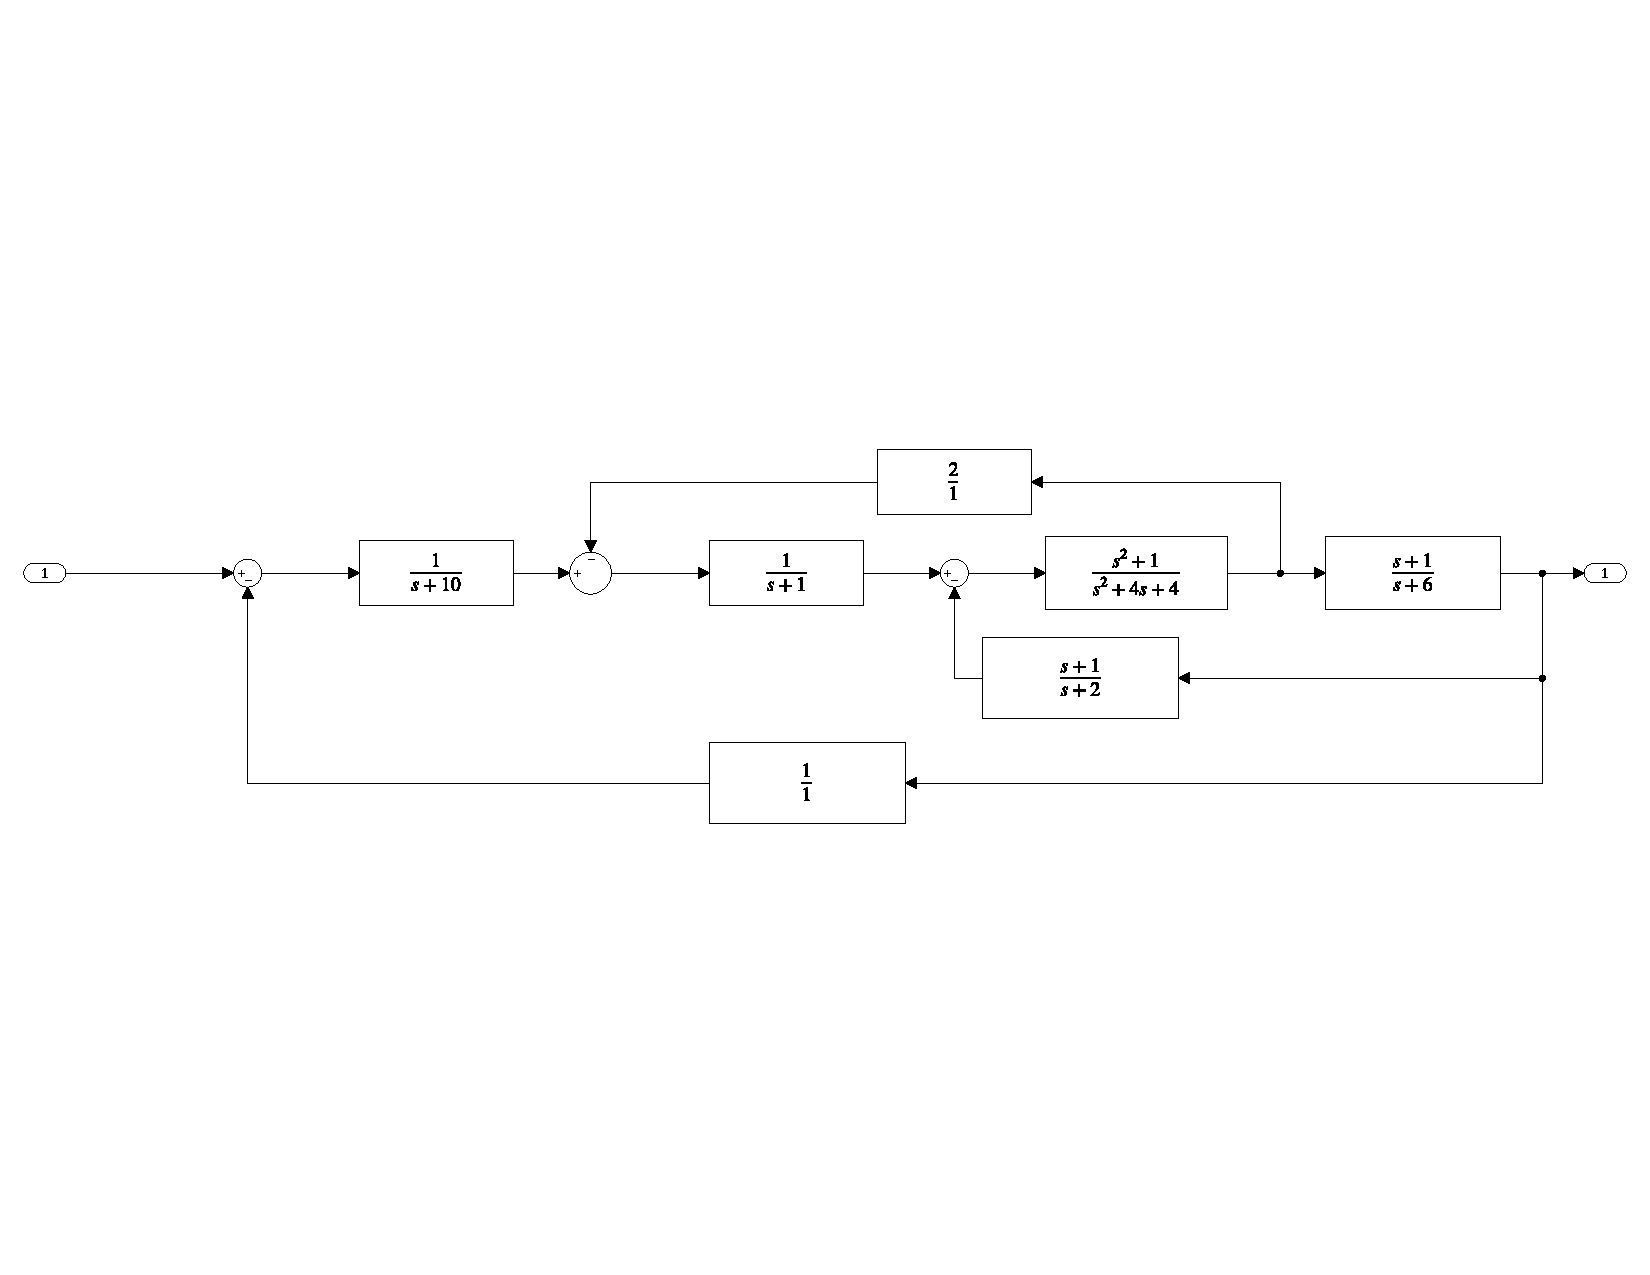
\includegraphics[width=0.8\linewidth]{system.pdf}
\end{center}
\caption{Sistema a analizar.}
\label{fig:system}
\end{figure}

Se puede observar como las funciones obtenidas por ambos métodos son idénticas.

\end{document}
